\documentclass{article}

\usepackage{graphicx}
%\usepackage{appendix}
%\usepackage{array}
\usepackage{siunitx}
\usepackage{authblk}	% prettier multiple authors
\usepackage{tikz}

\usepackage[margin=0.75cm]{caption}
\usepackage{hyperref}

% see http://texblog.org/2008/05/07/fwd-equal-cell-width-right-and-centre-aligned-content/
%\newcolumntype{x}[1]{%
%>{\centering\hspace{0pt}}p{#1}}%

\title{Trend Detection in Social Data}
\author[]{Scott Hendrickson}
\author[]{Jeff Kolb}
\author[]{Brian Lehman}
\author[]{Joshua Montague}
\affil[]{ \Large{Twitter, Inc.} }

\begin{document}
\maketitle

\frenchspacing

%%%%%%%%%%%%%%%%%%%%%%%%%%%%%%%%%%
\section{Introduction}
\label{intro}

Interactions in social data tell us about the real world. By
understanding the time-dependent behavior of groups of social media users, we
can identify and even predict important real-world trends. 

What sort of real-world activities, events, and trends might be reflected in
social data? And what properties of those events might we want to know?

Suppose an influential financial analyst tweets a strong opinion about a stock,
and the Tweet goes viral. Or suppose a large number of customers take to
Twitter to complain about a new product. In both cases, a good first question
is: when did the event happen, or when did the trend start? As a followup, we
can also ask: how significant is the change? How large is the increase or
decrease? More importantly, how large is the change relative to typical
changes? The quantification not only allows an analyst to distinguish the
atypical from the typical, but it also allows them to compare one atypical
event to another. Are there characteristics of the atypical events that allow
them to be separated into groups that can be assigned real-world meaning (e.g.
seasonal trends, holiday events)? If so, do these assignments point toward a
particular choice of model? If the identification of an atypical period of time
can be quantified, can it be automated? And can it be used to predict future
behavior?

After reading this paper, you will be well on your way to building a system to
discover, measure, compare and discuss changes in time series data that arise
from online social interactions.

%%%%%%%%%%%%%%%%%%%%%%%%%%%%%%%%%%
\section{Trends and Events}  \label{definitions}

We measure time-dependent user behavior with bucketed counts of mentions,
hashtags, followers, friends, links, or any quantity that can be counted over
time. If this quantity is defined by the presence of a word or phrase, that
word or phrase is called the \textit{topic}. When discussing changes in a
social data time series, we must speak concretely about what kinds of change
are interesting. For example, growth over time of an audience is a simple but
important measure of change. Similarly, we may want to know about seasonal
cycles of change. How does June compare to December? Against the backdrop of
steady growth and cyclic variations, we can ask about emerging changes, in
which a count rises from something negligible or unimportant to something
significant. We are also interesting in structural changes, where a time series
abruptly shifts from one state to another.

\subsection{Difficulties} Identifying growth, cycles, and especially emerging
and structural changes, is hard. Why? A primary difficulty is the fact that we
often don’t know in advance the scale or size of the change. The time interval
over which a change occurs can range from fractions of seconds to years, a
difference of 10 orders of magnitude! The size of the change can range from
counts of 10s through counts of billions. The community of users generating or
associated with the change can range from a single person through a group of
100 million people. It is difficult to construct algorithms that function
evenly over such broad ranges of data. Finally, we know that change of many
sorts is happening all the time, and we want to take care to identify single,
rather than composite, changes.

The corpus of social data is enormous, and this size brings about other
difficulties. Most signals of interest are relatively small.  Data that match a
particular topical filter are usually contaiminated by other signals, and
changes in the data reflect the cumulative result of all underlying effects.
The size of the data also implies the existence of many atypical patterns that
are entirely due to statistical variation, rather than reflecting real-world
events. Yet humans prefer to associate any changes with meaningful and
nameable events. 
%This is true whether the change is anticipated or not. 
Even
the distinction between the “real world” and the online social interactions is
complicated, and it can be
difficult to establish causality. Do the social data simply reflect the offline
world? How do online social interactions affect the rest of the world? 
The first step in unravelling this tangled feedback network is to 
qauntify the social data trends.  

\subsection{Analysis Trade-offs}
Attempts to quantify changes in social data are subject to trade-offs. 
At times, statistical noise in the data will be identified as a trend.
At other times, real trends will not be identified. We identify three 
particular measures of performance that account for these types of mistakes.
First is the \textit{time-to-detection}, or the time between the
real-world event and the detection in the social data. 
Second is the \textit{precision}, or the fraction of identified trends 
that are not statistical flukes. 
Last is the \textit{recall}, or the fraction of real trends that are identified
by the trend detection scheme.
These performance metrics can not be simultaneously optimized.
For example, if we wish to quickly identify an
emerging change, and we wish to do so with high confidence that we’re not
detecting random fluctuations, we will necessarily have 
low recall for real trends, and be 
able to only identify very statistically significant patterns.

\subsection{Classification}
Once the detection scheme is defined, humans have to interpret
and act on anomalous events as they are observed. These actions can take the
following forms:

\begin{itemize} 
    \item alerting - start paying attention to something new and urgent 
    \item informing - note the relative state of things available when someone 
        checks 
    \item discovery - do iterative refinement for novelty detections or root 
        cause analysis 
    \item model building - enable downstream consumption of the signal for 
        other modeling purposes 
\end{itemize}

Given these challenges and considerations, let’s organize the analysis around
three classes of anomalies, as seen in Figure~\ref{fig:anomalies}. While
anomolous decreases in time series can be interesting, we will limit ourselves
for the duration of the paper to the specific case of atypical increases.

\textbf{Ramp-up}: from a well-understood steady state (negligible, constant, or
periodic), the time series exhibits a continuing increase that is sustained
over many instances of the time resolution. 

\textbf{Mean shift}: from a well-understood steady state, the mean of the time
series shifts abruptly to a significantly different value and maintains that
value over a time span much longer than the time resolution. 

\textbf{Pulse}: from a well-understood steady state, the value of a time series
increases significantly, then returns to previously-typical values.
Pulses with widths similar to the time resolution capture the briefest
events that can be observed. Those with widths much larger than 
the time resolution represent extended events that can be further
characterized by the area under the pulse.

\begin{figure}[h]
\begin{center}
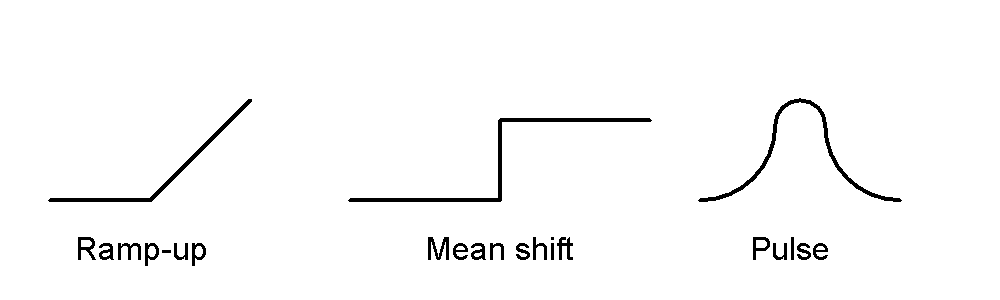
\includegraphics[width=0.95\textwidth]{fig/anomalies.png}
\caption{Three basic types of anomalies.}
\label{fig:anomalies}
\end{center}
\end{figure}

There is some interrelation between these basic anomaly types. For example, a
pulse can be thought of as a pair of mean shift or ramp-up/ramp-down anomalies.
A higher-level feature like a cycle can also be thought of as a sequence of
these anomalies. 
    
A final challenge is the mapping between anomalies and real-world events. The
word ``event'' can refer to a nameable change (e.g. Superbowl mentions), but it can
also refer to any interval in a time series that is sufficiently atypical, with
no meaning attached. In the remainder of this paper, we use the word event to
refer to specific, nameable happenings in the either the online or the offline world. 

We encourage the reader the systematically think about what sorts of change
are important to the problem they’re trying to solve, and what sorts of
action are to be taken upon detection. Identifying and characterizing
atypical behavior in social data time series can be difficult, but it it
provides us with brand-new insights into group behavior and the interplay
between the online and the offline world.  


%%%%%%%%%%%%%%%%%%%%%%%%%%%%%%%%%%%%%%%%%%%%%%%%%%%%%%%%%%%%%%%%%%%
\section{Brief Survey of Analytical Approaches}
\label{techniques}

In the section, we will work through the details of a simple technique for
trend detection in a time series defined by a topic on Twitter. We will then briefly
review a set of other techniques that extend, generalize, or improve on the
simple case. See the Appendix for a link to implementations of these
techniques.

Many techniques for identifying trending behavior define a background model,
which can be thought to represent the null hypothesis, or the case of “no
trend”. Deviations from the background model are described by a figure-of-merit
called $\eta$,
and large values of $\eta$ can be said to disprove the null hypothesis. 
In other techniques, the model includes both a background component and
and trend-like component. In these cases, the $\eta$ value quantifies the 
extent to which the data look more like a trend than a non-trend. 
Whatever the model, we say that the topic is trending at the time the
$\eta$ exceeds a pre-determined value. 

To calculate $\eta$, we typically must choose some model parameter values. 
If we have access to historical data that is labeled with truth 
(trend or no-trend) and the true trend start time, we
can measure the performance of a choice of model and parameter values, in terms
of the precision, the recall, and time-to-detection. 
%By recall, we mean the fraction of true trends that are identified by the algorithm. 
By time-to-detection, we mean the difference in time between the true start of
the trend and the first detection of it. 

%%%%%%%%%%%%%%%%%%%%%%%%%%%%%%%%%%
\subsection{Point-by-point Poisson Model}
\label{pbppm}

The Poisson distribution describes the probability of observing a particular
count of some quantity, when many sources have individually low probabilities
of contributing to the count. This sounds applicable to the case of counting in
social data, because each individual has a small chance of tweeting about a
given topic, but the large Twitter user base leads to significant counts. We
can do a rather simple form of trend detection by assuming that the counts in a
social data time series are Poisson-distributed around some average value, and
then looking for unlikely counts according to the Poisson model. Consider, for example,
the number of tweets in some time interval that contain the hashtagged phrase ``\#scotus''.
If we ignore variations in the overall rate of tweeting, we might expect the
counts of ``\#scotus''-containing tweets to vary, but the distributions of counts
will generally follow the Poisson distribution,
\begin{equation}
    P(c_i;\nu) = \nu^{c_i}\cdot e^{-\nu} / c_i!
\end{equation}
where $P$ is the probability of observing $c_i$ ``\#scotus'' tweets in the given time
window, when the expected number of such tweets is $\nu$. While we have no way of
knowing the true value of $\nu$, a good source is the time interval \textit{previous} to the
one being tested, $c_{i-1}$. We identify trends by counts $c_i$ that are particularly
unlikely, given the previous count, $c_{i-1}$, and the assumption of Poisson
distributed data. 

In this Poisson model, the unlikeliness of a particular count $c_i$ can be
quantified by the distance from the mean ($\nu$) in multiples of the confidence 
interval (CI) with confidence level $\alpha$. Confidence intervals for a Poisson mean $\nu$ and
confidence level $\alpha$ can be found in \cite{George:2012}. 
The parameter $\eta$ described the unlikeliness of a particular point:
\begin{equation}
    c_i = \eta \cdot \textrm{CI}(\alpha, \nu) + \nu, \textrm{where } \nu = c_{i-1}.
\end{equation}
In other words, a count $c_i$ is defined to
reject the null hypothesis when
\begin{equation}
    c_i >= \eta_c \cdot \textrm{CI}(\alpha, c_{i-1}) + c_{i-1},
\end{equation}
for predetermined values of $\eta_c$ and $\alpha$. 
The references in
the Appendix have code that produces high-precision estimates of the
Poisson confidence intervals. In Figure~\ref{fig:scotus1}, we plot the hourly counts for a
data set defined by the ``\#scotus'' hashtag. While there may be minor events
driving mentions of ``\#scotus'', this time series does not contain any major
real-world events, and the values of $\eta$ are relatively low.

\begin{figure} 
\begin{center}
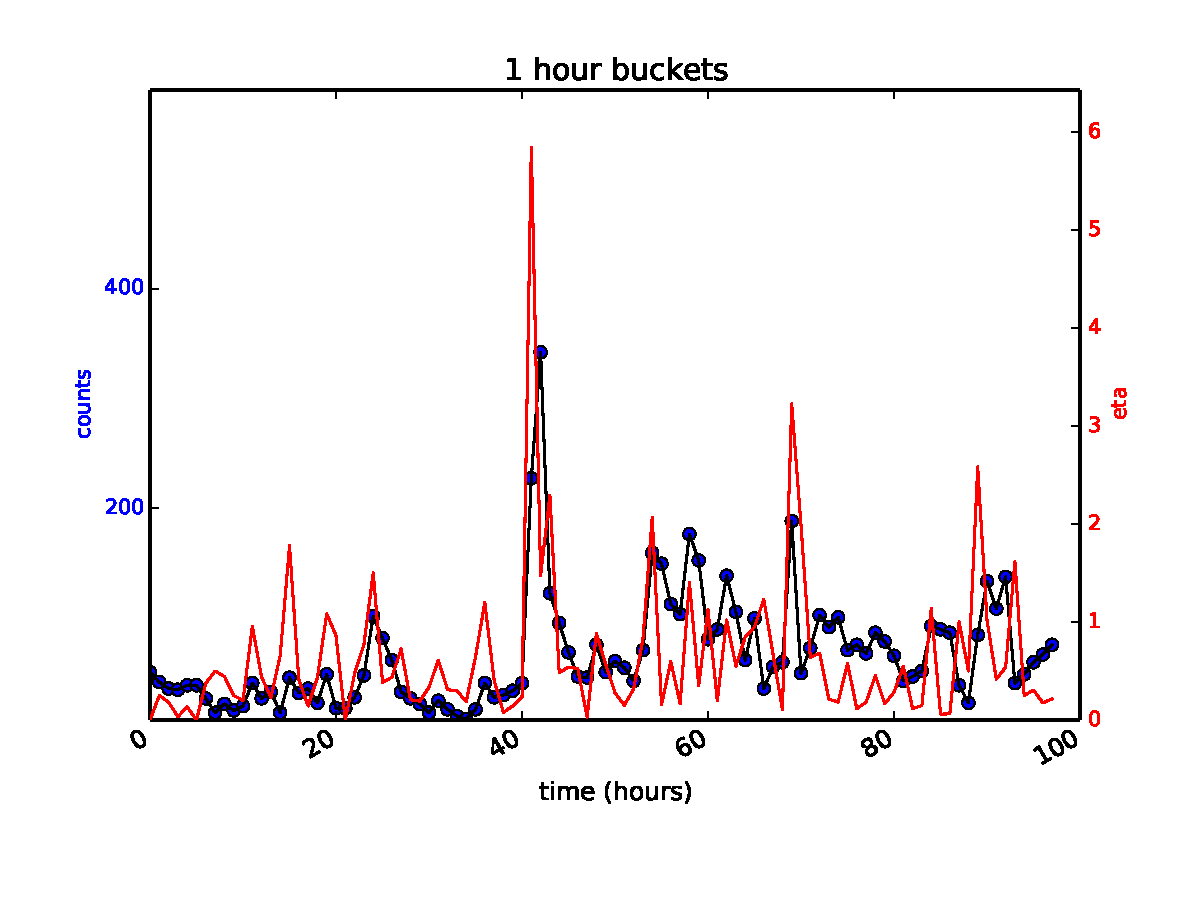
\includegraphics[width=0.95\textwidth]{fig/scotus_pbppm.pdf} \caption{Mentions
of ``\#scotus'' per hour. The time series data are shown in the blue dots with
black lines. For each point, $\eta$ is calculated based on the previous point, and
plotted in red. In this case, $\alpha=0.99$. }
\label{fig:scotus1}
\end{center}
\end{figure}

The point-by-point Poisson model is an attempt to simplify the problem of
background description by assuming a very simple model. Yet this
simplicity can be a source of challenges. First, we see that the data are
generally not Poisson-distributed around the previous data point. For example,
given a choice of $\alpha=0.99$, we should see values of $\eta>1$ only about 1\% of the
time. Still, the parameter $\eta$ is indicative of atypical counts, just not with
the usual probability interpretation. For example, Figure~\ref{fig:jobs} shows a time series with a
very distinctive, large spike, and the corresponding values of $\eta$ are very 
large.

\begin{figure}
\begin{center}
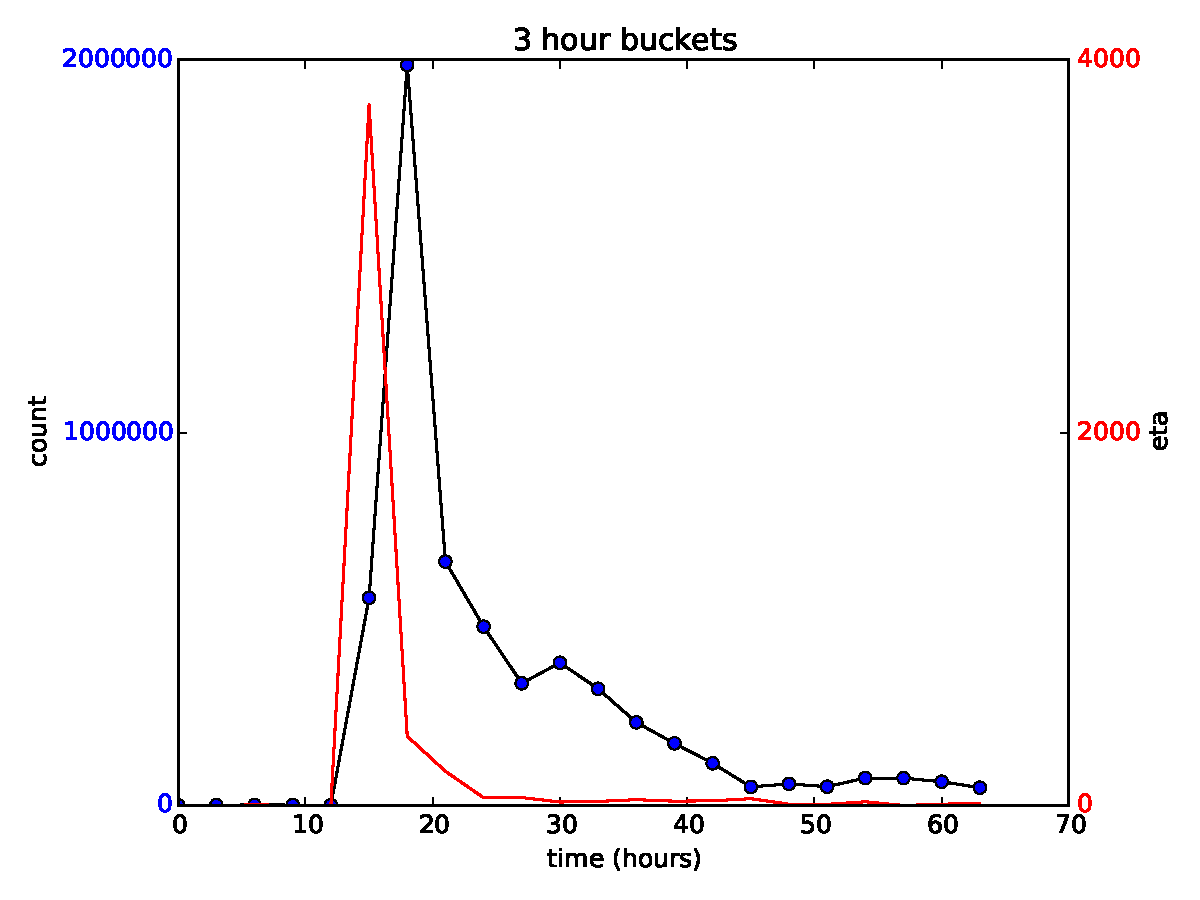
\includegraphics[width=0.95\textwidth]{fig/jobs.pdf}
\caption{Mentions per 3-hour intervals of “Steve Jobs”, around the time of his
death. The time series data are shown in the blue dots with black lines. For
each point, $\eta$ is calculated based on the previous point, and plotted in red.
In this case, $\alpha=0.99$. } 
\label{fig:jobs}
\end{center}
\end{figure}

Once a value of $\alpha$ is chosen, the definition and identification of a trend is
still dependent on the choice of two parameters values: $\eta_c$ and the time
interval for a single data point. As $\eta_c$ is increased, the precision is increased, 
but more real trends are missed (decreased recall). 
A similar trade-off exists for the bin width, as shown in
Figure~\ref{fig:scotus2}: small bins provide faster identification of trends, but lead to
worse precision.

\begin{figure}
\begin{center}
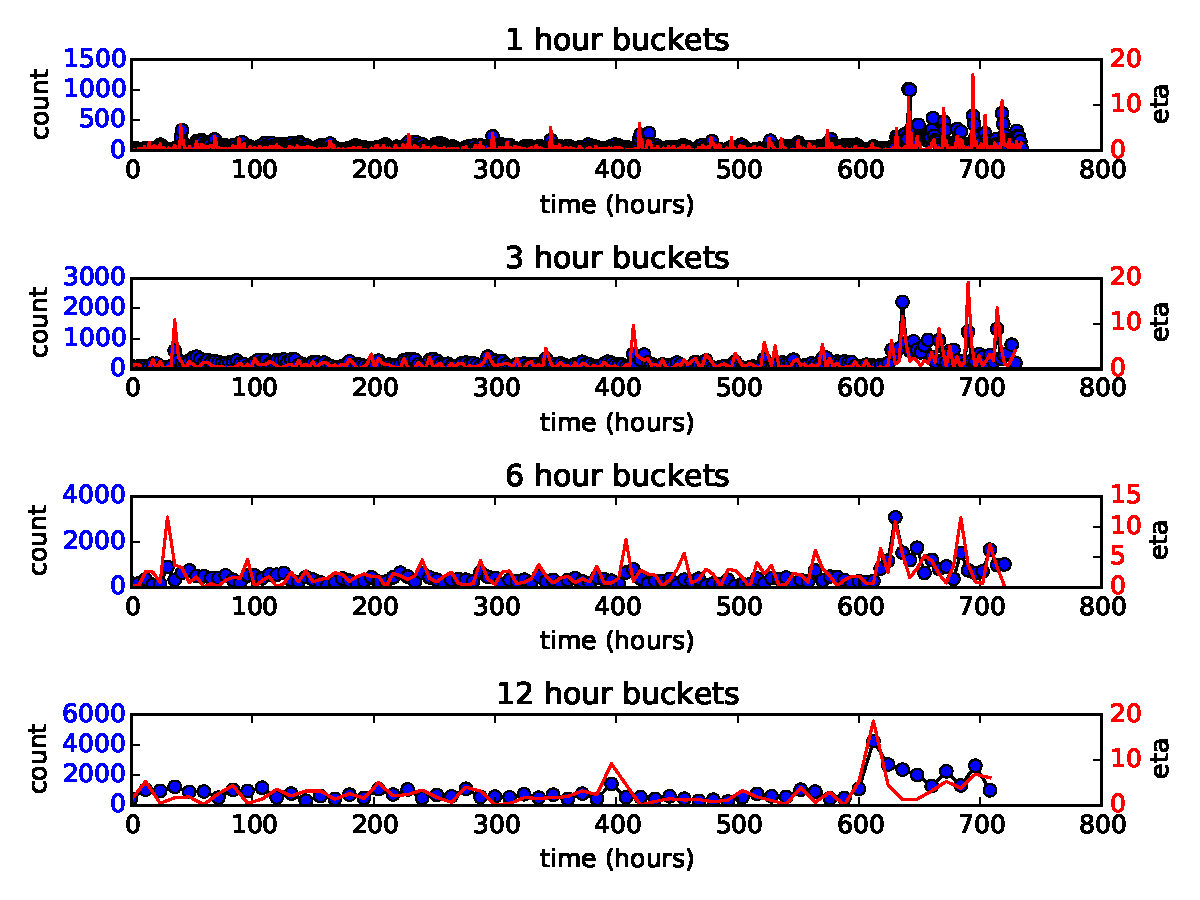
\includegraphics[width=0.95\textwidth]{fig/scotus_bucket_size.pdf}
\caption{Counts of ``\#scotus'' mentions, in variously-sized time buckets. The time
series data are shown in the blue dots with black lines. For each point, $\eta$ is
calculated based on the previous point, and plotted in red. In this case,
$\alpha = 0.99$.}
\label{fig:scotus2}
\end{center}
\end{figure}

Despite the challenge of choosing appropriate parameter values, the
point-by-point Poisson model can be very appealing. It's fast, in part
because it requires a single data point for the background model. It's also
easy to implement, and its single measure of atypicality, $\eta$, is fairly easy
to interpret. 

%%%%%%%%%%%%%%%%%%%%%%%%%%%%%%%%%%
\subsection{Cycle-corrected Poisson Model}
\label{ccpm}

Most social data time series exhibit cyclic patterns that reflect genuine human
cycles of activity. For example, if the majority of users that generate a
particular body of tweets live in a narrow band of time zones, we would
naturally expect to see fewer tweets during night hours for those time zones.
Thus, the patterns of hours, days, weeks, and even months can be reflected in
changes in rates of social media use. 

To reduce the rate of false trend identification due to expected, cyclic human
activity, the cycle-corrected Poisson model builds on the foundation of the
point-by-point Poisson model, and uses a background model derived from data
similar to the point being tested. For example, if a data point represents 3
hours of data from a Friday night in the Eastern US, it would not make a good
model to use the previous three hours as the Poisson mean. People tweet about
different topics at 2-5PM than they do at 5-8PM, leading to topical time series
with large variations simply due to the progression of the day. A better
background model for the data from 5-8PM on a particular Friday is an average
over the data from the 5-8PM interval on other days of the week. We can build
an even better model by taking the average over the same time interval, but
only from previous Fridays. If monthly cycles of activity are important, we
might even build our background estimate from only Fridays around the same time
of the month. 

The primary drawback of this technique, relative to the point-by-point model,
is the need to sample and retain enough data to calculate the background
estimates. If anomalous events have previously occurred in the time series,
this will contribute to the rolling averages and artificially increase the rate
of false positives. Figures~\ref{fig:scotus3} and \ref{fig:scotus4} shows a comparison of the two Poisson-based
background model discussed in this and in the previous section. The
cycle-corrected model shows generally reduced $\eta$ values (fewer false
positives), but actually produces a greater $\eta$ value at the initial spike
around Sept. 20. 

\begin{figure}
\begin{center}
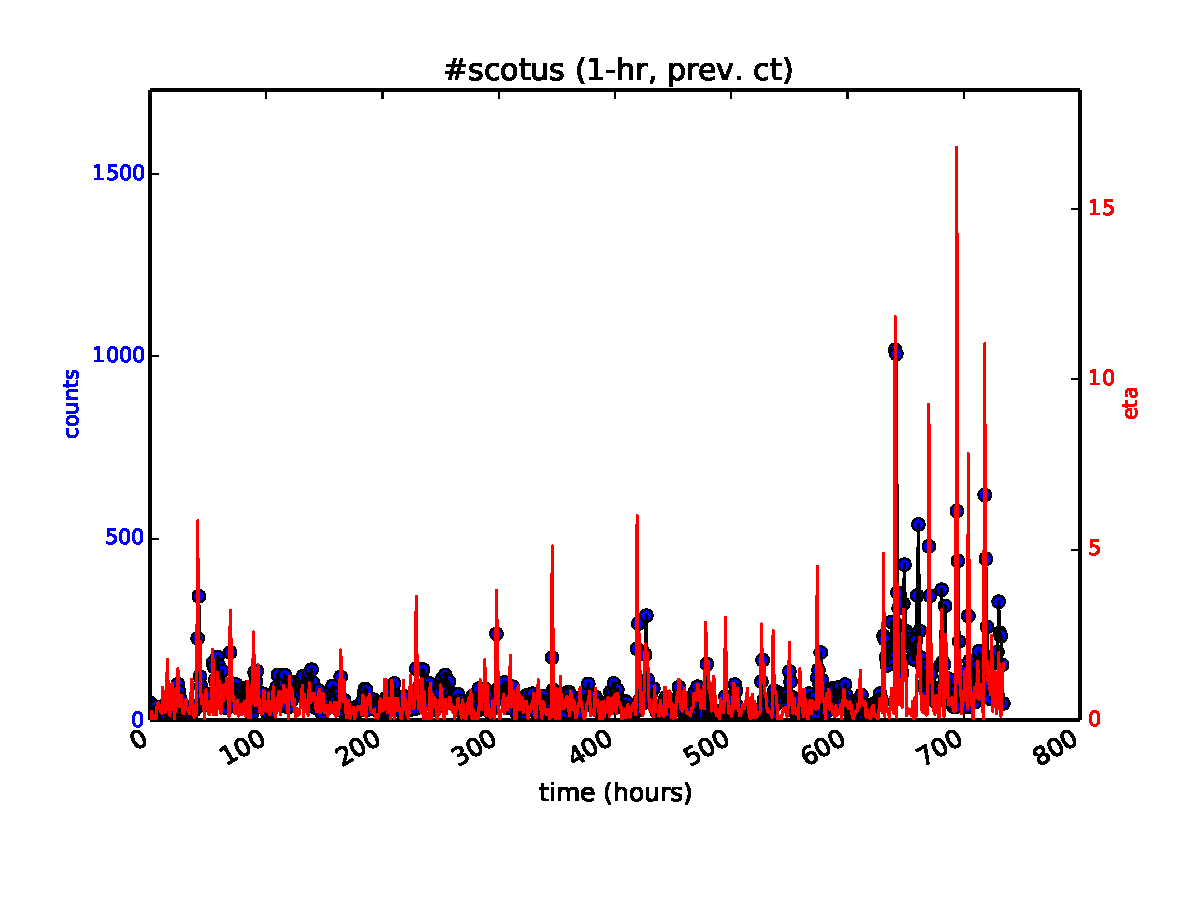
\includegraphics[width=0.95\textwidth]{fig/scotus_1month_pbppm.pdf}
\caption{Counts of ``\#scotus'' mentions, in 1-hour time buckets. The time series
data are shown in the blue dots with black lines. For each point, $\eta$ is
calculated based on the previous point, and plotted in red. In this case, 
$\alpha=0.99$.} \label{fig:scotus3}
\end{center}
\end{figure}

\begin{figure}
\begin{center}
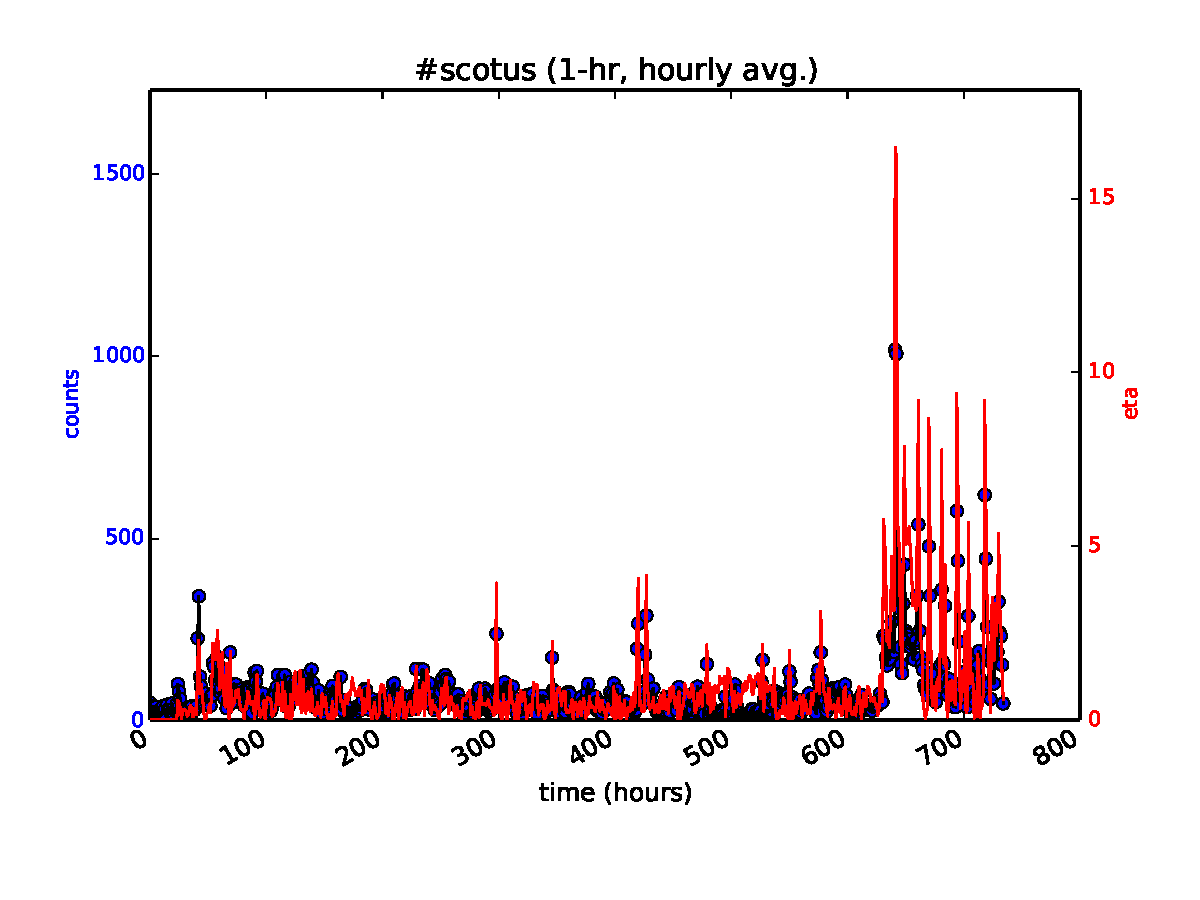
\includegraphics[width=0.95\textwidth]{fig/scotus_1month_ccpm.pdf}
\caption{Counts of ``\#scotus'' mentions, in 1-hour time buckets. The time series
data are shown in the blue dots with black lines. For each point, $\eta$ is
calculated based on the average value from the same hour on previous days
in the time series, and plotted in red. In this case, $\alpha=0.99$. }
\label{fig:scotus4}
\end{center}
\end{figure}

Continuing to expand on the basic Poisson model, there is a variety of
further improvements that can be made. Any value chosen for the Poisson
mean can be further stabilized by calculating an average over a rolling
window of adjacent data points. If the long-term overall growth rate for
the data is known, this baseline can be subtracted from the
data. Ihler, Hutchins, Smyth \cite{Ihler:2006} present a
framework for removing the effects of previously-occurring anomalies from
the Poisson background model. 



%%%%%%%%%%%%%%%%%%%%%%%%%%%%%%%%%%
\subsection{A Data-driven Method} 
\label{nikolov}

There is a two-fold drawback to the Poisson models: first, it is impossible to
choose a value for $\eta_c$ that is a good choice for trends of all shapes
and sizes. Moreover, our decision to use the Poisson distribution as a model
for the variations in the data is not necessarily a good choice. In fact, we
know that many social data time series are not Poisson-distributed. What if we
were to avoid these problems by simply comparing the data to real examples of
trending and non-trending data?

Nikolov suggests we do just this in a non-parametric method \cite{Nikolov:2011}. We
begin by compiling a library of labeled time series, identifying each as
trending or non-trending. We then define a weight that is a function of the
distance between a labeled time series and the data in question. The final
result is simply the ratio of the total weight for the trending time series
divided by the total weight for the non-trending time series. 

We start by collecting \textit{reference} time series from historical data. Based on their
shape and the details of real-life events associated with them, we label
them “$+$” (trending) or “$-$” (non-trending). The sets of references time
series are named $R+$ and $R-$, and typically haves sizes in the 100s. 
In general, the elements of $R+$ and $R-$ are much 
longer than the time series that they are compared to. 

We next define a distance between two same-length time series: $d(r,s)$,
where $r$ is in $R+$ or $R-$ and $s$ is the time series that we’re evaluating for
trending behavior. To facilitate comparison, both time series are unit-normalized. 
We use the Euclidean distance:
\begin{equation}
    d(r,s) = \Sigma_i^N(r_i - s_i)^2,
\end{equation}
where $r_i$ and $s_i$ are the $i$-th points in the $N$-length time series $r$ and $s$. Other
choices of distance functions emphasize different properties of the
time series, and lead to different value of the trend detection metrics
discussed below. If $r$ is longer than $s$, we define the distance to be the
smallest of all distances $d(r_s,s)$, where $r_s$ is any $s$-length sub-series of $r$. Given
a distance function, we then define a weight in terms of a scaling
parameter $\lambda$. 
\begin{equation}
    W(r,s) = e^{-\lambda\cdot d(r,s)}
\end{equation}
We then sum up the weights from the trending and non-trending comparisons and
produce a final metric from their ratio:
\begin{equation}
    \eta(s) = \frac{\Sigma_{r\in R+}W(r,s)}{\Sigma_{r\in R-}W(r,s)} 
\end{equation}
To demonstrate the performance of this technique on a known trend,
Figure~\ref{fig:nikolov_eta} shows a plot of an element of R+ ($s+$), along with $\eta$.
The $\eta$ curve rises dramatically soon after the real spike in the
data, with the lagtime demonstrating the effect of the data-smoothing.

\begin{figure}
\begin{center}
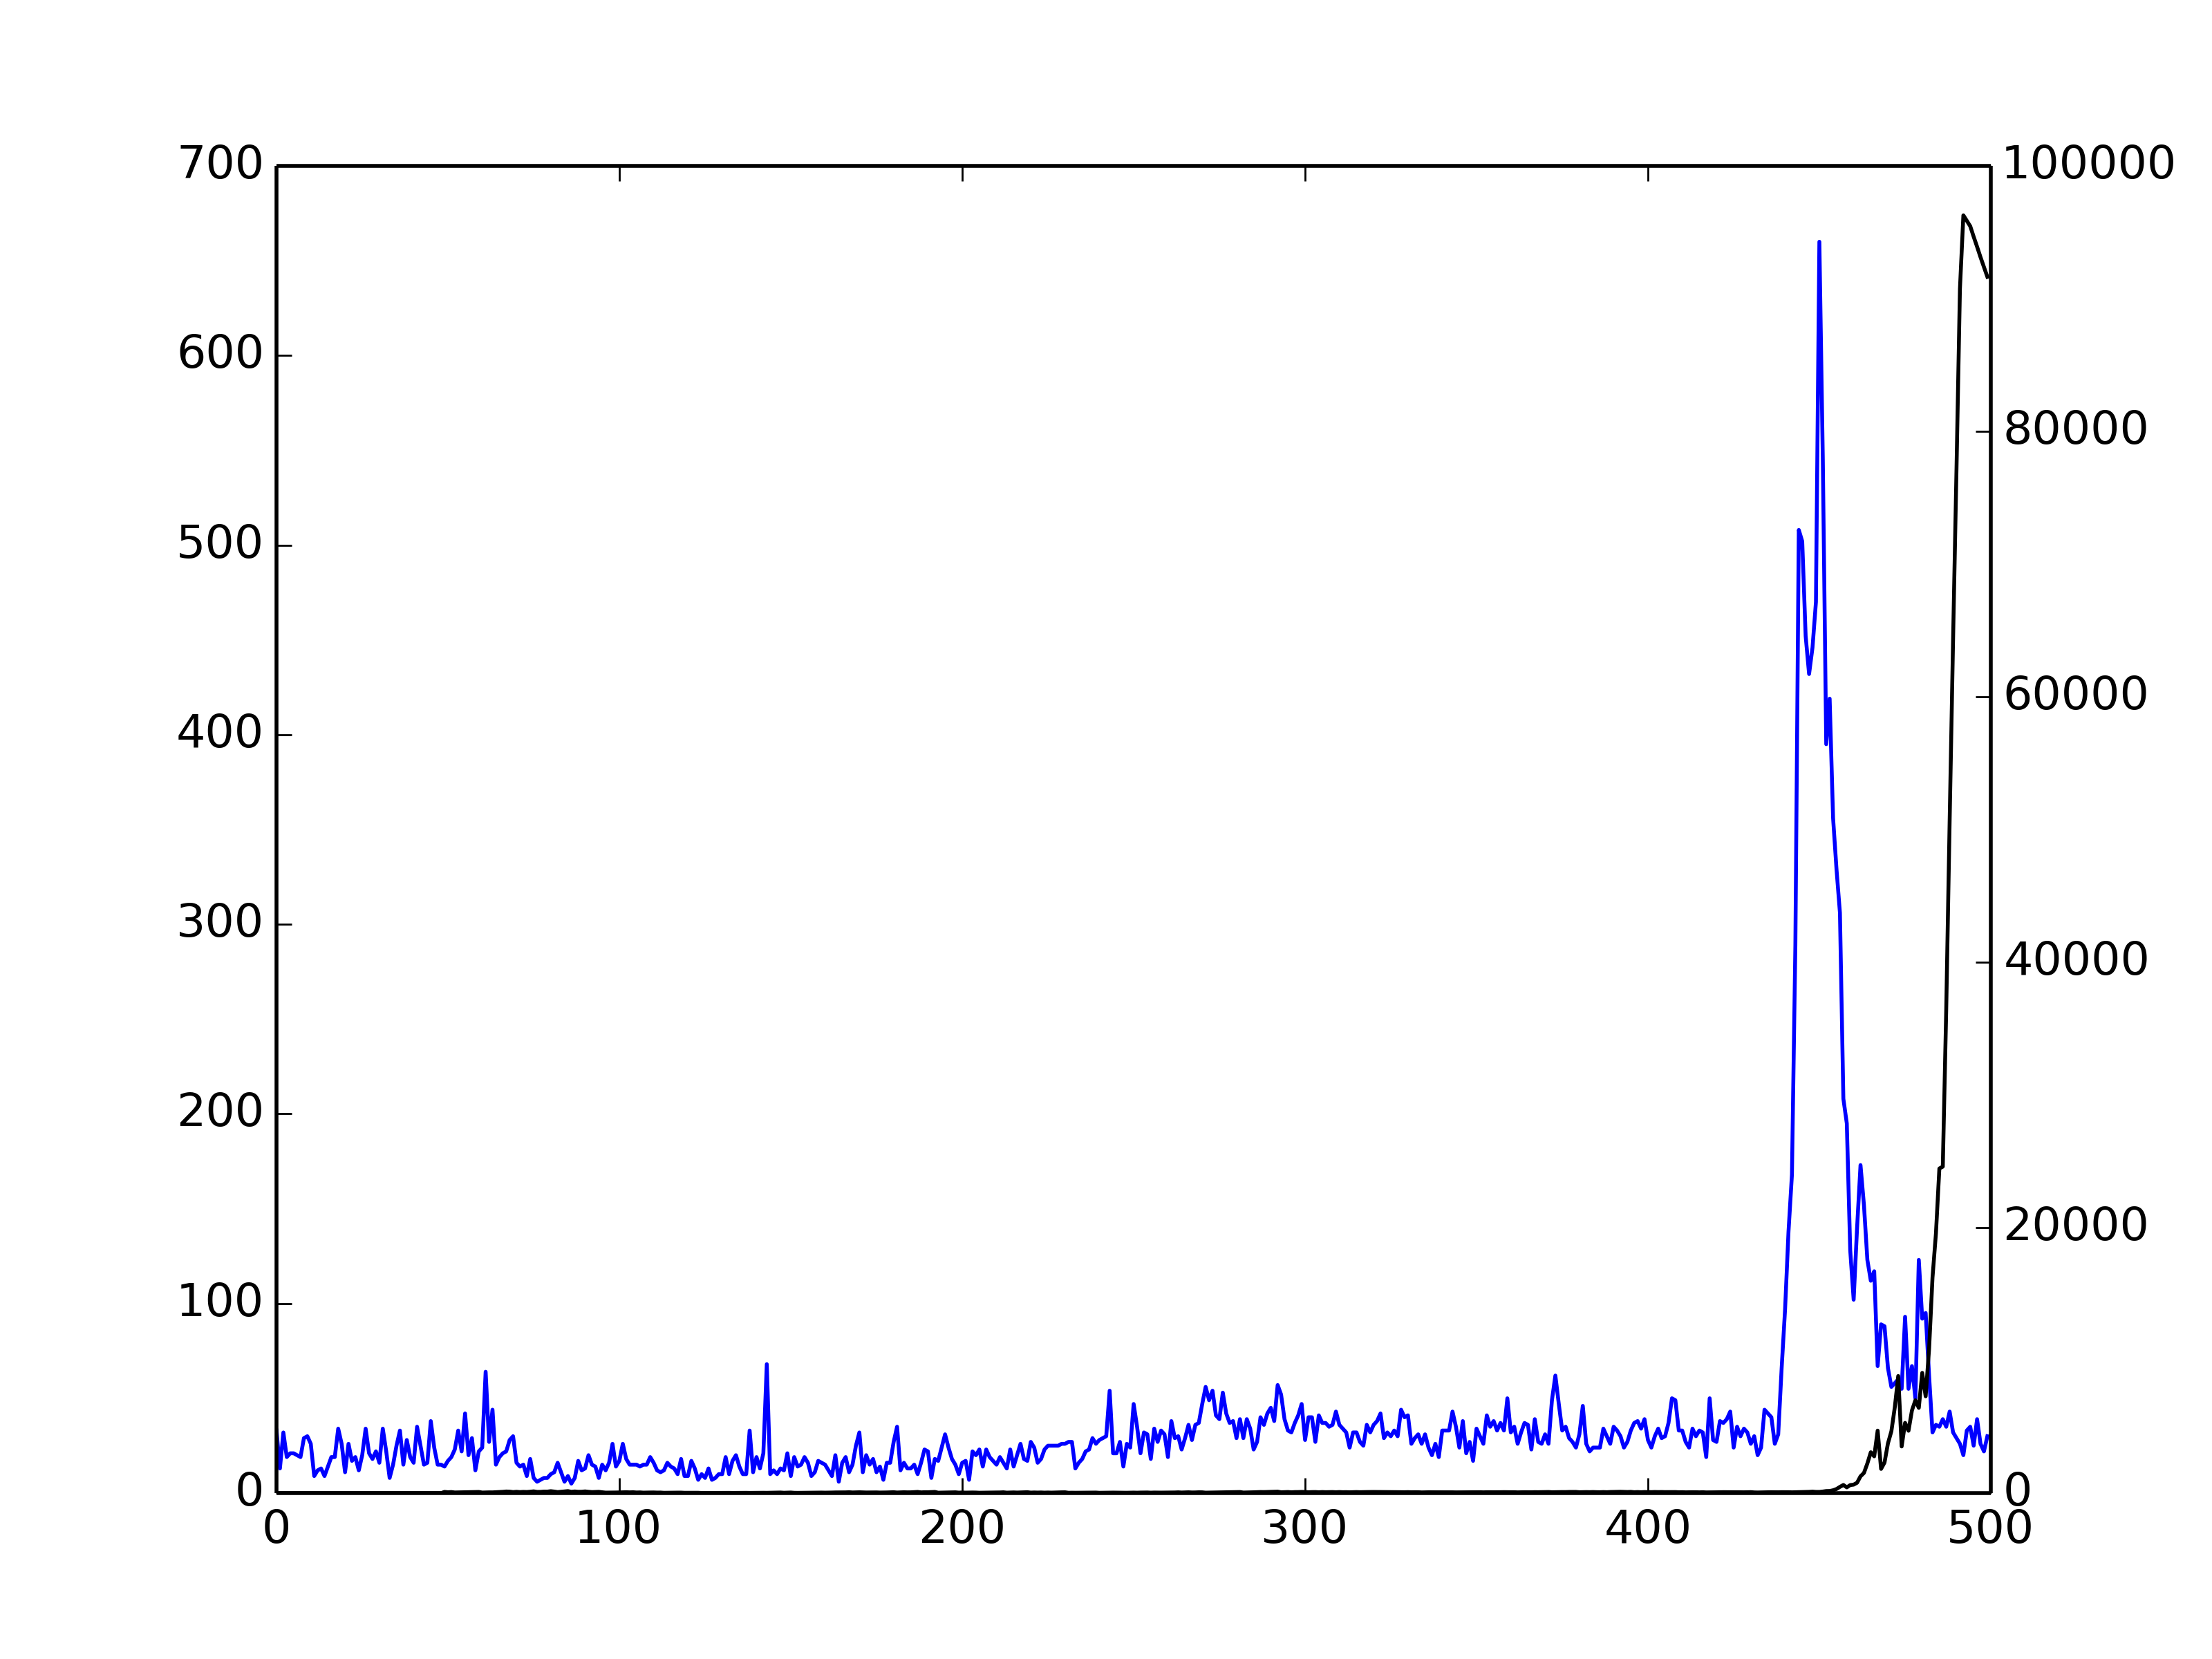
\includegraphics[width=0.95\textwidth]{fig/nikolov.png} 
\caption{Data from a reference time series in $R+$ are plotted in blue, for
2-minute time intervals. Based on a library of 500 reference trends in $R+$
(minus the one being tested) and 500 reference non-trends in $R-$, the figure of
merit $\eta$ is calculated for each point and plotted in black. The length of
elements of $R$ is 200 minutes, while the length of the tested series ($s$) is 100
minutes. 
%For distance calculations, the data are smoothed over a 40 minute window.
}
\label{fig:nikolov_eta} 
\end{center}
\end{figure}

The primary difficulty with this method is the need for a labeled set of reference time
series. To obtain similar detection performance over a broad range of trend shapes and sizes, 
it is also important to apply a series of transformations to all $r$ and $s$.
In our implementation, these transformation include the previously-mentioned unit normalization, 
a smoothing with an average taken over a sliding window,
and a logarithmic scaling
(see \cite{Nikolov:2011} or the code referenced in the Appendix
for details of the transformations). 
Examples of the transformed reference time series are shown in Figure~\ref{fig:reference_series}.

\begin{figure}
\begin{center}
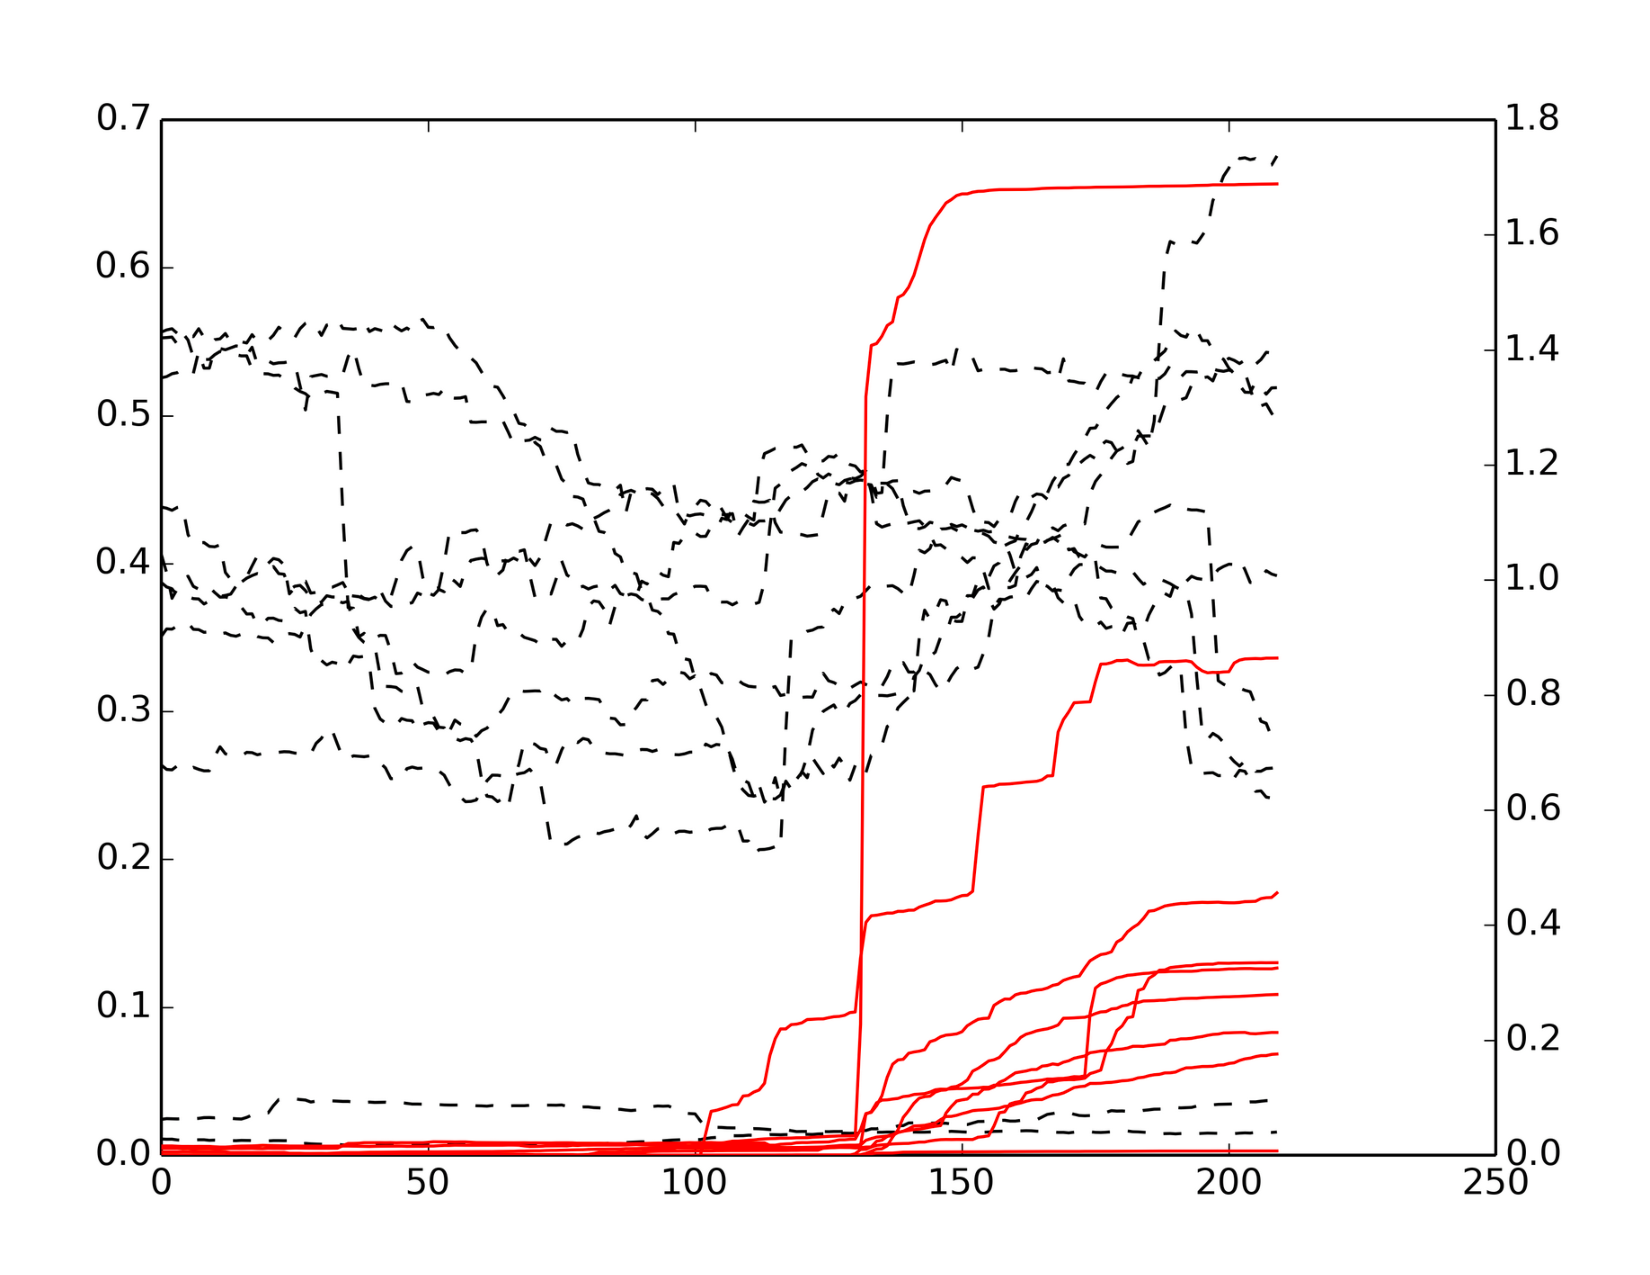
\includegraphics[width=0.95\textwidth]{fig/nikolov3.pdf} 
\caption{A plot of elements of $R+$ (red lines) and $R-$ (black dashed lines), 
after the smoothing and scaling described in~\cite{Nikolov:2011}.  
The trending series in $R+$ rise sharply at the right side of the plot, 
while changes in series in $R-$ are more evenly distributed.}
\label{fig:reference_series}
\end{center}
\end{figure}

%Once a reference library is created and the transformations defined, this setup can be used
%for any future analysis. 
%The performance of this algorithm is controlled by the values of
Even though the shapes of the labeled time series provide the model for
trending and non-trending time series, the analyst still controls the performance
of the algorithm by setting parameter values.
%must choose the time resolution and length of those
%series. The analyst must also choose an appropriate value for the scaling
%parameter and define any other transformations applied to the time series. 
The values chosen for the scaling parameter, the lengths of $s$ and $r$, time series
precision, and any other transformation parameters lead directly to the
precision and recall metrics. With the labeled reference series
in hand, we can easily calculate these metrics by removing a single
element from $R+$ or $R-$ and testing it against the ensemble. 


%%%%%%%%%%%%%%%%%%%%%%%%%%%%%%%%%%%%%%%%%%%%%%%%%%%%%%%%%%%%%%%%%%%
\section{Conclusion} 

Trends in social data tell us about what is important to users of social media.
Trends not only reflect real-world events, but also drive offline behavior. By
identifying trending behavior, we can be informed of current events, we can
discover emerging events, and we can model future events. But reliable,
precise, and fast trend detection is made difficult by the size and diversity
of the social data corpus, along with the large variations in the time and
volume scales of social data sets. 

We have overviewed three techniques of trend detection that strike various
balances between simplicity, speed, accuracy, and precision.
If simplicity is extremely important, or for a pilot model, we
recommend the point-by-point Poisson technique. This technique is most
appropriate to small sets of time series, in which typical behavior can be
manually observed and correlated with the atypicality parameter ($\eta$). If a 
sufficient history of data is available, we recommend enhancing the technique
to account for cyclic behavior, as in the cycle-corrected Poisson technique.
This is a relatively small step up in complexity, and provides a significantly
decreased rate of false positive signals. 

When optimal coverage and false positive rates are worth extra model complexity
and technical commitment, we recommend using the data-driven method. While it
is potentially difficult to collect and label a sufficient number of comparison
time series, the technique provides stable results across a wide variety of
trend detection problem. 


\appendix
\section{Appendix}
The latest version of this document 
and implementations of the trend detection models 
can be found at:
\noindent \url{https://github.com/jeffakolb/Gnip-Trend-Detection}.

%If you find errors in this work, or have comments, please email jkolb\@twitter.com. This 
%work is licensed under a Creative Commons Attribution-ShareAlike 3.0 Unported License:
%
%\noindent \url{http://creativecommons.org/licenses/by-sa/3.0/deed.en_US}.

%%%%%%%%%%%%%%%%%%%%%%%%%%%%%%%%%%%%%%%%%%%%%%%%%%%%%%%%%%%%%%%%%%%


\begin{thebibliography}{2013}

\bibitem{George:2012} F. George B. Golam Kibria, \textsl{Confidence
    Intervals for Signal to Noise Ratio of a Poisson Distribution},
    \url{http://thescipub.com/abstract/10.3844/amjbsp.2011.44.55} 2013.

\bibitem{Ihler:2006} Ihler, Hutchins, Smyth, \textsl{Adaptive Event
    Detection with Time–Varying Poisson Processes},
    \url{http://www.datalab.uci.edu/papers/event_detection_kdd06.pdf} 2006.

\bibitem{Nikolov:2011} S. Nikolov, \textsl{Trend or No Trend: A Novel
    Nonparametric Method for Classifying Time Series},
    \url{http://dspace.mit.edu/bitstream/handle/1721.1/85399/870304955.pdf}
    2011.  

\end{thebibliography}

\end{document}
